% !TeX root = ../main.tex
\section{Methods}
\label{sec:methods}

% “数据怎么进来、算法怎么评估、消融和 benchmark 怎么做、最后怎样得到 turnover history”；
We developed a workflow to reconstruct recurrent balsa stand disturbances from near-decadal Sentinel-1 observations and translate the detected events into plantation turnover histories (Fig.~\ref{fig:workflow}). The analysis comprised four stages: construction of track-specific stand-level time series, recurrent-event detection with the proposed Windowed CUSUM, spatially structured evaluation and sensitivity analysis, and reconstruction of disturbance recurrence and inter-disturbance intervals. All data preprocessing, detection, evaluation, and statistical analyses were implemented in Python 3.12.

% ====================================================
\subsection{Track-specific Sentinel-1 trajectory construction and stand representation}
\label{sec:s1_timeseries_representation}
% ====================================================

Track-specific monthly Sentinel-1 time series were organized using the Sentinel-1 Gridded Time Series (S1-GRiTS) data-cube framework (\url{https://github.com/ottoKae/S1-GRiTS}). S1-GRiTS preserves pass direction, relative orbit, and polarization as explicit indexing dimensions. For each calendar month $t$, all valid burst-level RTC backscatter observations contributing to the same grid cell, track, and polarization were summarized by their median. The resulting monthly gridded data cube therefore retained separate time series for each track and polarization, with observations from different acquisition geometries kept separate.

% track-specific 不是为了数据管理方便，而是为了让后面的 local-reference assumption 更合理。
As shown in Fig.~\ref{fig:workflow}(a), the monthly grids were subsequently converted to stand-level trajectories using the mapped balsa polygons. For the primary Polygon-first representation, all finite grid-cell values whose centres fell within a polygon were aggregated by their spatial median for each month. We refer to this strategy as Polygon-first because spatial aggregation was performed before disturbance detection. This produced one monthly trajectory for each polygon, track, and polarization. Track identity was retained so that each temporal sequence was constructed under a consistent acquisition geometry, providing an internally comparable temporal background for subsequent local-reference change detection.

Alternative representations were evaluated to determine whether detection performance depended on the spatial aggregation strategy. Polygon-first alternatives included the spatial mean, histogram mode, and a representative grid cell. Pixel-first alternatives retained individual grid-cell trajectories through disturbance detection and subsequently consolidated candidate evidence using connected eight-neighbour support, temporal DBSCAN, or joint space--time DBSCAN~\citep{Ester1996DBSCAN}. Because Pixel-first approaches do not form a single stand trajectory before detection, they require additional spatial-support or clustering parameters, which were selected exclusively from spatial training data as described in Section~\ref{sec:experimental_evaluation}. 


% =====================================================

\subsection{The proposed Windowed CUSUM}
\label{sec:windowed_cusum}

% “这个算法解决什么问题、设计原则是什么、核心模块是什么”。
% 聚焦说明核心设计原则：temporal adaptation + statistical adaptation

Building on the geometry-consistent trajectories described above, Windowed CUSUM was designed to detect recurrent disturbances under temporally heterogeneous Sentinel-1 backgrounds. For such trajectories, disturbance evidence should be interpreted relative to both a dynamically renewed local background and the variability of that background, because backscatter levels and temporal variability can differ among stands and evolve through time. Windowed CUSUM therefore adapts at two levels. Overlapping local-reference windows repeatedly renew the temporal context as each stand evolves, while a window-specific permutation null calibrates each observed CUSUM amplitude against the variability of that same local context. This design avoids reliance on a fixed historical baseline and does not require recursive segmentation after each detected event. Within each window, candidate timing and direction are identified and statistically screened. Accepted candidates are then consolidated across overlapping windows and Sentinel-1 tracks to form a recurrent stand-disturbance history (Fig.~\ref{fig:windowed_cusum_concept}).


\begin{figure*}[pos=!htbp]
    \centering
    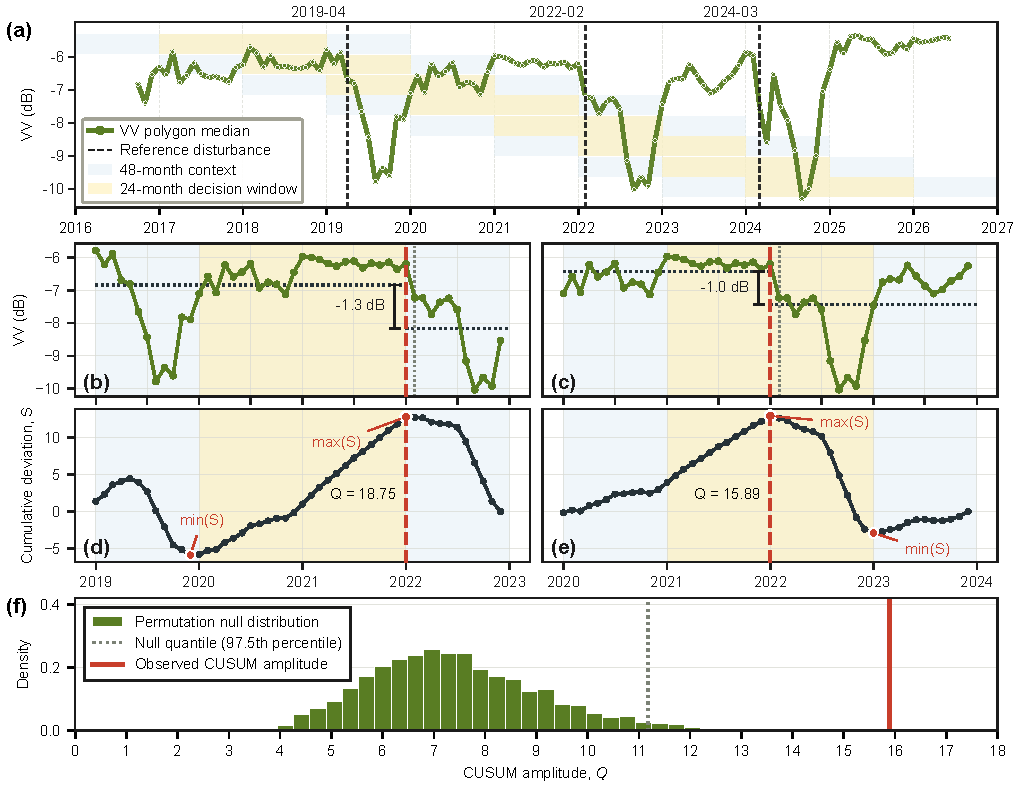
\includegraphics[width=\linewidth]{figures/fig04_windowed_cusum_concept.pdf}
    \caption{Conceptual illustration of Windowed CUSUM for one balsa stand.
    (a) Near-decadal stand-level monthly VV trajectory with reference disturbances and overlapping local-reference windows, showing the temporal context and central decision intervals.
    (b,c) CuSum computation within each window, where candidate points are identified from the maximum cumulative deviation.
    (d,e) Corresponding cumulative-deviation curves, with candidate locations identified from the maximum cumulative residual. The candidate in (d) is rejected because it falls outside the decision interval, whereas that in (e) is retained.
    (f) Evaluation of the retained CUSUM amplitude against its window-specific permutation null.}
    \label{fig:windowed_cusum_concept}
\end{figure*}


% ----------------------------------------------------
\subsubsection{Local temporal adaptation within overlapping windows}
\label{sec:windowed_cusum_windows}
% ----------------------------------------------------
% 当前应该和哪个背景比较？
% 为什么需要局部 temporal reference
% W, S, W_b, D_b
% 为什么 estimation context 和 event admission 分开
% boundary / missing observations / locked W,S

A stand trajectory can contain repeated disturbance and recovery, so a reference defined over the complete record may no longer represent the stand's current condition. Windowed CUSUM therefore evaluates each track-specific trajectory through overlapping local contexts, repeatedly renewing the temporal reference without permanently segmenting the series after an earlier detection. Let $T$ denote the length of the available monthly calendar, $W$ the nominal context-window length, and $S$ the displacement between consecutive windows. For a nominal window beginning at month $b$, the observed context window and its decision window were defined as Equation~\eqref{eq:window_definition}.
\begin{equation}
    \mathcal{W}_b
    =
    [\max(0,b),\,\min(T,b+W)),
    \qquad
    \mathcal{D}_b
    =
    [\max(0,b+S),\,\min(T,b+W-S)),
    \label{eq:window_definition}
\end{equation}
with half-open intervals expressed in calendar months. For interior windows, the central decision window has length $C=W-2S$, requiring $W>2S$.

The two intervals serve different purposes. All finite observations within $\mathcal{W}_b$ contribute to estimation of the local CUSUM, providing temporal context on both sides of a potential transition. Candidate events are admitted only when their estimated month falls within $\mathcal{D}_b$. This central-admission rule reduces sensitivity to transitions estimated near artificial window boundaries, where temporal support is asymmetric. Thus, displacement of $\mathcal{W}_b$ provides temporal adaptation, while $\mathcal{D}_b$ restricts event reporting to the better-supported portion of each local context.

The locked operational configuration used $W=48$ months and $S=12$ months, yielding a 24-month central decision interval for interior windows. Alternative values of $W$ and $S$ were evaluated in the configuration-sensitivity analysis (Section~\ref{sec:experimental_evaluation}). Context windows were clipped to the available record without temporal padding and were subject to the same candidate-admission rules. Each window required at least 12 finite observations, and missing months retained their original calendar positions without interpolation or temporal shifting.

% ----------------------------------------------------
\subsubsection{Local CUSUM candidate characterization}
\label{sec:windowed_cusum_candidate}
% ----------------------------------------------------

Within each local context window, CUSUM was calculated from the finite observations in chronological order. Let $x_1,\ldots,x_n$ denote these observations and $\bar{x}$ their mean. The centred cumulative residual and CUSUM amplitude were defined as Equation~\eqref{eq:local_cusum}, where $n$ is the number of finite observations in the window.
\begin{equation}
    S_t
    =
    \sum_{i=1}^{t}(x_i-\bar{x}),
    \qquad
    Q
    =
    \max_t S_t-\min_t S_t,
    \qquad
    t=1,\ldots,n,
    \label{eq:local_cusum}
\end{equation}
where $S_t$ represents the accumulated departure from the local window mean and $Q$ summarizes the strength of the dominant temporal departure within that window. The window mean serves only as a local centring reference and is not interpreted as an independently known undisturbed-canopy baseline.

For the sustained negative shifts targeted in this study, positive residuals tend to accumulate before the decline and negative residuals afterward, causing the cumulative residual to reach a maximum near the transition between the two states. The candidate location was therefore defined as Equation~\eqref{eq:candidate_position}~\citep{Page1954CUSUM,Ygorra2021CuSum}.
\begin{equation}
    t^*
    =
    \arg\max_t S_t ,
    \label{eq:candidate_position}
\end{equation}
with the first maximum retained in the event of a tie. The index $t^*$ was mapped back to its original calendar month before testing membership in the central decision interval $\mathcal{D}_b$. Candidates outside $\mathcal{D}_b$ were not admitted.

To determine the direction of the candidate change, $x_{t^*}$ was treated as the first post-change observation and the corresponding segment means were
\begin{equation}
    \bar{x}_{\mathrm{pre}}
    =
    \operatorname{mean}(x_1,\ldots,x_{t^*-1}),
    \qquad
    \bar{x}_{\mathrm{post}}
    =
    \operatorname{mean}(x_{t^*},\ldots,x_n).
    \label{eq:time_pre_post_mean}
\end{equation}

Both segments were required to contain at least one finite observation, and only candidates satisfying $\bar{x}_{\mathrm{post}} < \bar{x}_{\mathrm{pre}}$ were retained for statistical calibration. Thus, each local candidate was characterized by its CUSUM amplitude $Q$, candidate month $t^*$, and direction of change. 
% The reported month represents an algorithmic transition boundary at monthly resolution and is not interpreted as the exact physical onset of disturbance.

% ----------------------------------------------------
\subsubsection{Window-specific statistical calibration}
\label{sec:windowed_cusum_permutation}
% ----------------------------------------------------

The raw CUSUM amplitude $Q$ measures the strength of temporal organization within a local window, but its absolute value is not directly comparable across stands or windows. Sentinel-1 background variability can differ with canopy condition, moisture, seasonality, and acquisition geometry~\citep{BorlafMena2023Seasonality,vanDerWoude2024S1Disturbance}. A common threshold on $Q$ could therefore represent very different levels of evidence in a temporally stable stand and in a highly variable stand.

Windowed CUSUM instead calibrates each observed amplitude against a null distribution generated from the same local observations. For each eligible window, the finite observations were randomly reordered while preserving their values and sample size. This procedure retains the local marginal distribution and overall amplitude of backscatter variability while removing its observed temporal ordering. The CUSUM amplitude was then recalculated for each permutation. Let $Q_{\mathrm{obs}}$ denote the observed amplitude and $Q_j^{\mathrm{perm}}$ the amplitude obtained from permutation $j$. For $B$ permutations, the finite-sample-corrected permutation $p$ value was calculated in Equation~\eqref{eq:permutation_pvalue}~\citep{PhipsonSmyth2010Permutation}.
\begin{equation}
    p_{\mathrm{perm}}
    =
    \frac{
    1+\sum_{j=1}^{B}
    \mathbf{1}
    \left\{
    Q_j^{\mathrm{perm}}
    \geq
    Q_{\mathrm{obs}}
    \right\}
    }{B+1},
    \label{eq:permutation_pvalue}
\end{equation}

where $\mathbf{1}\{\cdot\}$ denotes the indicator function. A small $p_{\mathrm{perm}}$ indicates that an amplitude at least as large as $Q_{\mathrm{obs}}$ is rarely reproduced when the same local backscatter values are present but their temporal ordering is removed. Consequently, the same raw $Q$ can receive different statistical support in different windows because its interpretation is conditional on the variability of the corresponding local trajectory.

The initial calibration used $B=3{,}999$ permutations. Candidates with initial $p_{\mathrm{perm}}$ values between 0.015 and 0.035 were recalculated using $B=19{,}999$ permutations to improve Monte Carlo precision near the operational decision threshold. Candidates were statistically supported when $p_{\mathrm{perm}}\leq0.025$. Deterministic candidate-specific random seeds were used to ensure reproducibility.

The permutation $p$ value quantifies candidate-level evidence under the specified within-window randomization null. It is not interpreted as a posterior probability of disturbance or as global false-discovery control across overlapping windows. Independent permutation also removes short-range temporal dependence and therefore assumes exchangeability under the null. Sensitivity to alternative null formulations that preserve temporal dependence was evaluated separately in Section~\ref{sec:experimental_evaluation}.

Futhurmore, candidates passing the directional and statistical screening were still window-level, track-specific nominations. Because overlapping windows could nominate the same transition repeatedly and different Sentinel-1 tracks could localize the same disturbance to adjacent months, accepted candidates were consolidated within each polygon and polarization. Nominations occurring within one month were grouped into the same temporal event cluster; repeated nominations from the same track did not add support. The representative month was selected by the greatest number of supporting distinct tracks, with the earliest month retained under ties. This produced one ordered polygon-level event sequence per polarization. VV and VH remained separate through detection and consolidation, while polarization configurations were evaluated independently in Section~\ref{sec:experimental_evaluation}.


% % ---------------------------------------------------------------
% \subsubsection{Candidate consolidation into recurrent stand histories}
% \label{sec:windowed_cusum_consolidation}
% % ---------------------------------------------------------------

% Candidates passing the directional and statistical screening remained window-level, track-specific nominations rather than unique disturbance events. The same physical disturbance could be nominated repeatedly by overlapping windows, while independent Sentinel-1 tracks could localize that disturbance to adjacent calendar months because of differences in acquisition timing and local temporal context. Accepted candidates were therefore consolidated before constructing polygon-level recurrent disturbance histories.

% Consolidation was performed separately within each polygon and polarization. Candidate nominations occurring within one month of one another were grouped into the same temporal event cluster. Repeated nominations from overlapping windows on the same track did not contribute additional track support. For each cluster, the representative event month was selected as the month supported by the greatest number of distinct Sentinel-1 tracks, with the earliest month retained when distinct-track support was tied.

% This procedure removed repeated window-level nominations and reconciled small timing differences among track-specific detections to produce a single ordered event sequence for each polygon and polarization. VV and VH were processed independently through detection and consolidation, without averaging the two polarization trajectories. The choice of polarization configuration, including VV-only, VH-only, union, and cross-polarization agreement, was evaluated separately in the sensitivity analysis described in Section~\ref{sec:experimental_evaluation}.



\subsection{Disturbance-history reconstruction}
\label{sec:history}

We counted consolidated detections during 2017--2025. For polygon $m$, the ordered consolidated disturbance months were denoted $H_m=(h_{m,1},\ldots,h_{m,n_m})$, where $n_m$ is the number of detected events. Stand-level recurrence was summarized by $n_m$. For stands with at least two events, consecutive inter-disturbance intervals were
\begin{equation}
    R_{m,k}=h_{m,k+1}-h_{m,k},
    \qquad k=1,\ldots,n_m-1.
\end{equation}
Only adjacent detected events were paired, so no interval was constructed across an intermediate event. The pooled interval distribution weighted individual intervals equally. Spatial recurrence was summarized in fixed 10-km-wide hexagons using the median polygon event count, including zeros; hexagons without inventory polygons were left unclassified.


% ====================================================
\subsection{Experimental design and accuracy assessment}
\label{sec:experimental_evaluation}
% ====================================================

Evaluation was organized to separate reference-based detector assessment from configuration selection, component attribution, benchmark comparison, and temporal robustness analyses. 
% A common spatially structured inference framework was used throughout, while parameter selection was restricted to spatial training folds and locked configurations were not retuned during subsequent comparisons.

% ----------------------------------------------------
\subsubsection{Reference-event protocol and spatial inference}
\label{sec:reference_spatial_inference}
% ----------------------------------------------------

Historical signal characterization was separated from detector evaluation. Absolute backscatter distributions used all valid polygon--month observations from the 3,498 validated balsa polygons. Event-aligned analyses used independently interpreted reference events with month-level timing. For each polygon--track event, the pre-event background was summarized over months $-12$ to $-3$ and required at least six finite observations, whereas the event/post-event response used months 0 to $+2$ and required at least two. Track-specific responses were aggregated within each polygon event so that each disturbance contributed once. These criteria retained 1,018 events for paired and event-aligned signal analyses, while all 1,093 reference events from 462 polygons were retained for detector evaluation.

The 1,093 reference events were grouped into 57 spatial blocks and assigned to five event-balanced outer folds, with each polygon and all associated tracks and events kept within the same block. Parameters were selected using four folds and applied once to the held-out fold; predictions from the five held-out folds were then pooled to obtain spatial out-of-fold estimates~\citep{Roberts2017SpatialCV}. 
% Fixed-configuration analyses did not reopen parameter selection.

Detected and reference events were matched one-to-one within a prespecified $\pm2$-month tolerance, first maximizing the number of matches and then minimizing total absolute temporal lag. Let $N_{\mathrm{match}}$, $N_{\mathrm{pred}}$, and $N_{\mathrm{ref}}$ denote the numbers of matched events, predicted events, and reference events, respectively. Event-level precision, recall, and F1 were defined as
\begin{equation}
    Precision=\frac{N_{\mathrm{match}}}{N_{\mathrm{pred}}},
    \qquad
    Recall=\frac{N_{\mathrm{match}}}{N_{\mathrm{ref}}},
    \qquad
    F_1=\frac{2 \times Precision \times Recall}{Precision + Recall}.
    \label{eq:detection_metrics}
\end{equation}

Temporal accuracy was summarized only for matched events as
\begin{equation}
    \mathrm{MAE}
    =
    \frac{1}{N_{\mathrm{match}}}
    \sum_{i=1}^{N_{\mathrm{match}}}
    \left|\hat{t}_i-t_i\right|,
    \label{eq:temporal_mae}
\end{equation}

where $\hat{t}_i$ and $t_i$ are the detected and reference months of matched event $i$. Because the reference catalogue was not assumed to contain every historical disturbance, unmatched predictions were treated as unmatched relative to this catalogue rather than independently verified false disturbances.

Confidence intervals were estimated from 5,000 bootstrap resamples of the 57 complete spatial blocks, using identical resamples for paired method or configuration contrasts~\citep{Davison1997Bootstrap}.


% ----------------------------------------------------
\subsubsection{Configuration sensitivity and component attribution}
\label{sec:configuration_component}
% ----------------------------------------------------

Configuration sensitivity assessed stand representation, window geometry, and polarization. Under the locked $48/12$-month geometry and $p_{\mathrm{perm}}\leq0.025$, the Polygon-first median was compared with different spatial aggregation strategies metioned in Section~\ref{sec:s1_timeseries_representation}. Window sensitivity evaluated $W\in\{24,36,48,60,72\}$ months and $S\in\{6,12\}$ months, excluding 24/12 because $W-2S=0$, with geometry selected in training folds and evaluated on the held-out fold. Polarization sensitivity compared VV-only, VH-only, either-polarization, and VV--VH agreement under the retained representation and geometry.

Component attribution used the locked configuration. Progressive ablation started from a single-pass full-record CUSUM~\citep{Page1954CUSUM} and sequentially added local-reference windowing, central-interval admission, negative-direction screening, and window-specific permutation calibration; only the complete detector was termed Windowed CUSUM. Complementary removal tests omitted one component at a time while holding all other processing and evaluation choices fixed. Paired F1 contrasts used spatial-block resampling, with Holm adjustment for the four prespecified progressive contrasts. Reference polygons were additionally stratified by recorded event count to test whether local-reference windowing was most beneficial under recurrent disturbance.

% ----------------------------------------------------
\subsubsection{Benchmark comparison and statistical robustness}
\label{sec:benchmark_robustness}
% ----------------------------------------------------

Benchmarks used the same reference events, Polygon-first trajectories, missing-data treatment, event matching, and five-fold spatial outer-fold design. Method-specific parameters were selected only from training folds. Comparators included maximum monthly decline, classical lower CUSUM~\citep{Page1954CUSUM}, ReCuSum~\citep{Ygorra2023ReCuSum}, a BOCD prototype~\citep{Bottani2026f-pol_BOCD}, monthly CuSum NRT~\citep{Ygorra2024CuSumNRT}, and Continuous Change Detection and Classification (CCDC)~\citep{Bullock2022CCDC_S1}.
%  Where applicable, decrease-filtered variants imposed the same negative pre--post direction constraint without retuning.

The CuSum NRT core was checked against the initial implementation before adaptation to monthly stand-level trajectories. CCDC used the Earth Engine implementation with VV as the breakpoint band and optical TMask screening disabled. The BOCD implementation was treated as a benchmark adaptation rather than a full reproduction of the published detector. All benchmark outputs entered the same track-consolidation and event-matching procedure. The two prespecified primary F1 contrasts, Windowed CUSUM versus monthly CuSum NRT and CCDC VV, used 97.5\% confidence intervals for Bonferroni family-wise coverage of 95\%; other contrasts used exploratory 95\% intervals.

Statistical robustness was assessed by changing only the temporal null while keeping Windowed CUSUM fixed. The independent-value permutation was compared with the archived empirical-rank implementation, 3-, 6-, and 12-month calendar-block permutations, residual moving-block-bootstrap nulls~\citep{Kunsch1989BlockBootstrap}, and a track-wise maximum-statistic null. Stochastic nulls were repeated across ten random seeds. These analyses tested sensitivity to temporal-dependence assumptions and did not reopen detector selection.


% ----------------------------------------------------
\subsubsection{Temporal truncation and prospective replay}
\label{sec:temporal_prospective}
% ----------------------------------------------------

Temporal truncation evaluated how much post-event observation was required for stable detection. For each historical reference event, the Sentinel-1 record was truncated at 0, 1, 2, 3, 6, and 12 months after the reference month, and the locked Windowed CUSUM configuration was rerun using only observations available by each cutoff. No later observations were available to window construction, statistical calibration, candidate consolidation, or track fusion. Recall and event-date stability were evaluated on the 1,065 events with sufficient temporal support at every horizon, and uncertainty was estimated using the same spatial-block resampling procedure.

A separate prospective replay used observations available through June 2026 after all detector choices had been frozen. The 2026 manual review was excluded from representation, window, threshold, component, and benchmark selection. Because review was conditioned on detector-generated candidates, this analysis estimated candidate precision and operational behaviour but could not estimate missed disturbances or population recall.